\documentclass{standalone}
\usepackage[calc]{picture}
\usepackage{graphicx,transparent,color,amsmath,amssymb,amsfonts,tikz}
\graphicspath{Fig_SIM_subfigs}
\setlength{\unitlength}{1in}

\begin{document}


\begin{picture}(4.85, 3.2)(0.25,-3.2)

\put(0.5, -0.7){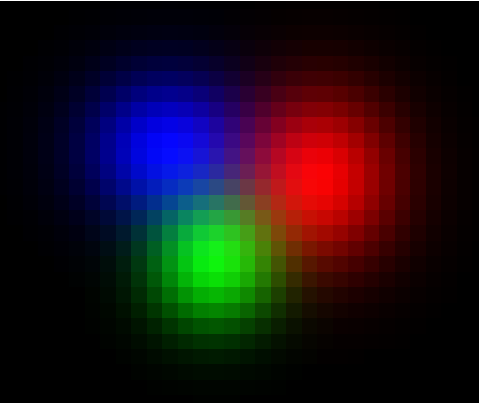
\includegraphics[height=0.6in]{Fig_SIM_subfigs/example_spatial_true.pdf}}
\put(1.1, -0.7){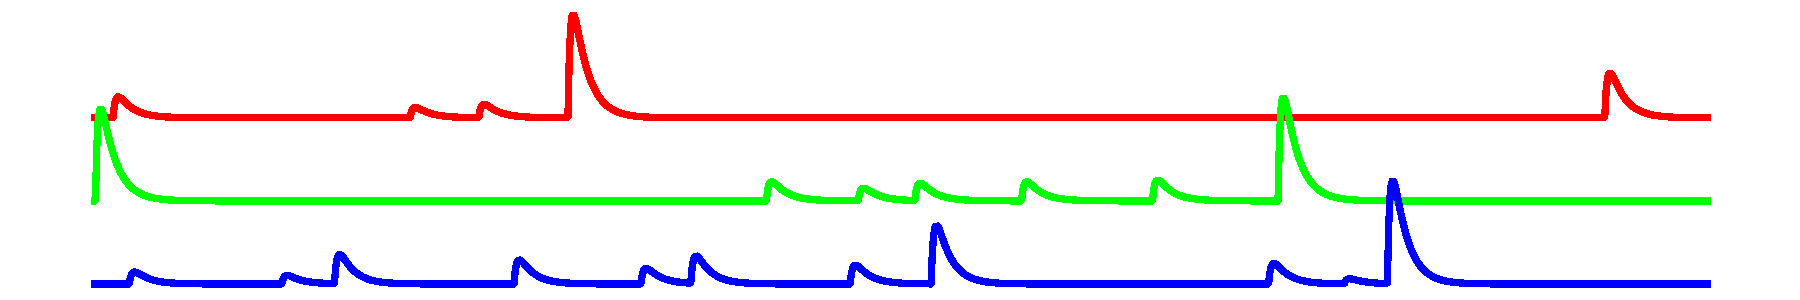
\includegraphics[height=0.65in, width=4.0in]{Fig_SIM_subfigs/example_temporal_true.pdf}}
\put(0.45,-0.75){\color{black}\line(1,0){4.6}}
\put(0.45,-0.75){\color{black}\line(0,1){0.7}}
\put(5.05,-0.75){\color{black}\line(0,1){0.7}}
\put(0.45,-0.05){\color{black}\line(1,0){4.6}}
\put(0.275, -0.65){\large\rotatebox{90}{\textbf{Truth}}}

\put(0.5, -1.5){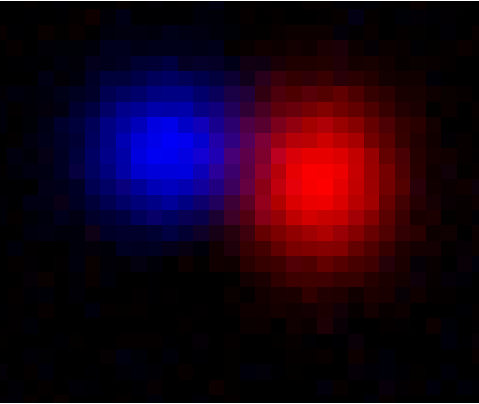
\includegraphics[height=0.6in]{Fig_SIM_subfigs/example_spatial_ica.pdf}}
\put(1.1, -1.5){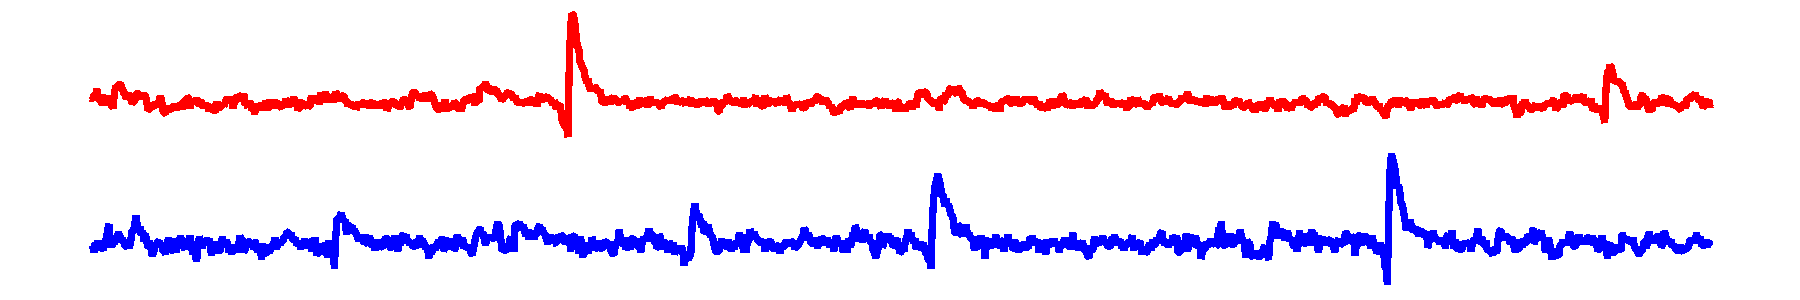
\includegraphics[height=0.65in, width=4.0in]{Fig_SIM_subfigs/example_temporal_ica.pdf}}
\put(0.45,-1.55){\color{black}\line(1,0){4.6}}
\put(0.45,-1.55){\color{black}\line(0,1){0.7}}
\put(5.05,-1.55){\color{black}\line(0,1){0.7}}
\put(0.45,-0.85){\color{black}\line(1,0){4.6}}
\put(0.275, -1.625){\large\rotatebox{90}{\textbf{PCA/ICA}}}

\put(0.5, -2.3){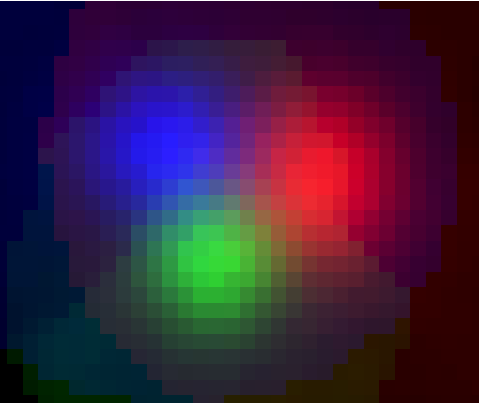
\includegraphics[height=0.6in]{Fig_SIM_subfigs/example_spatial_cnmf.pdf}}
\put(1.1, -2.3){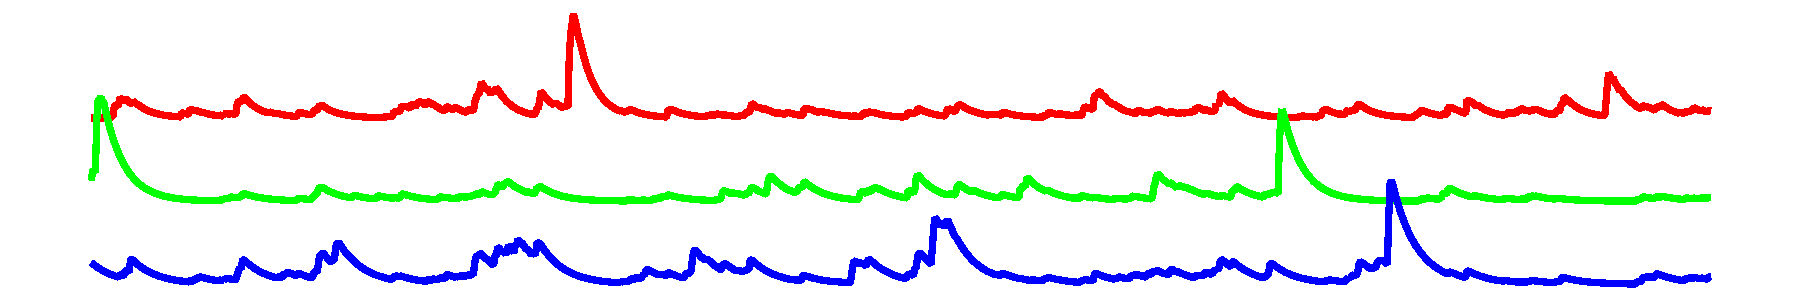
\includegraphics[height=0.65in, width=4.0in]{Fig_SIM_subfigs/example_temporal_cnmf.pdf}}
\put(0.45,-2.35){\color{black}\line(1,0){4.6}}
\put(0.45,-2.35){\color{black}\line(0,1){0.7}}
\put(5.05,-2.35){\color{black}\line(0,1){0.7}}
\put(0.45,-1.65){\color{black}\line(1,0){4.6}}
\put(0.275, -2.28){\large\rotatebox{90}{\textbf{CNMF}}}

\put(0.5, -3.1){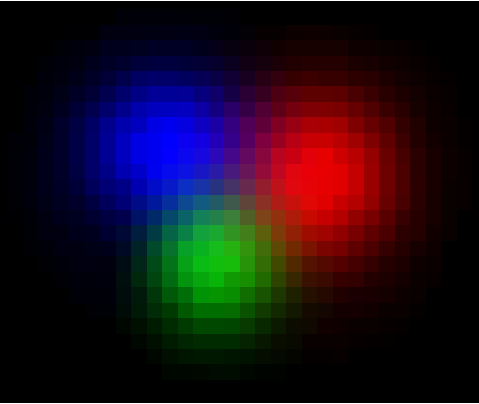
\includegraphics[height=0.6in]{Fig_SIM_subfigs/example_spatial_cnmfe.pdf}}
\put(1.1, -3.1){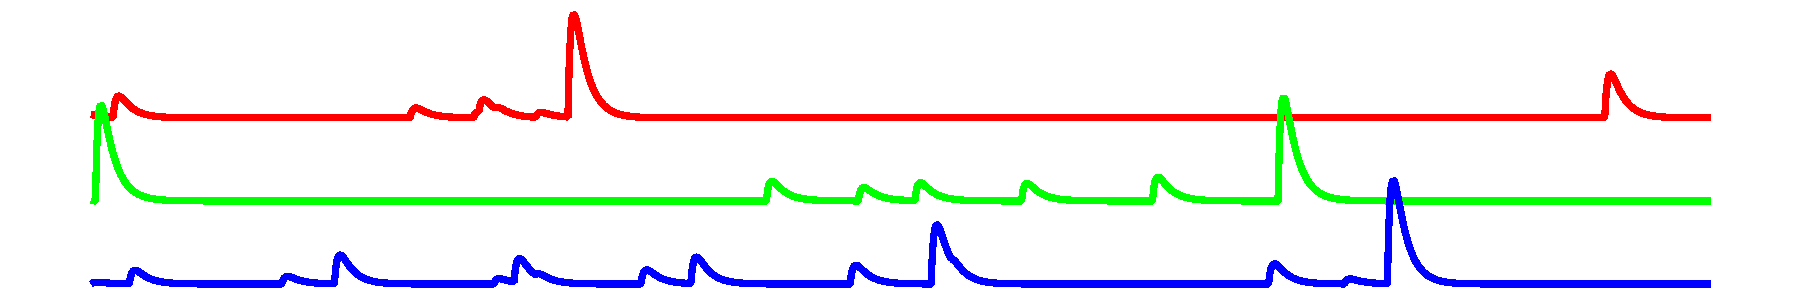
\includegraphics[height=0.65in, width=4.0in]{Fig_SIM_subfigs/example_temporal_cnmfe.pdf}}
\put(0.45,-3.15){\color{black}\line(1,0){4.6}}
\put(0.45,-3.15){\color{black}\line(0,1){0.7}}
\put(5.05,-3.15){\color{black}\line(0,1){0.7}}
\put(0.45,-2.45){\color{black}\line(1,0){4.6}}
\put(0.275, -3.18){\large\rotatebox{90}{\textbf{CNMF-E}}}
\end{picture}
\end{document}
